\documentclass[pdf]{article}
%\usepgfplotslibrary{external} 
%\tikzexternalize 
\usepackage{tikz} 
\usepackage{enumerate}
\usepackage{graphicx,psfrag}
\usepackage{amsmath} 
\usepackage{subcaption}
  \DeclareRobustCommand{\squaret}[1]{\tikz{\draw[#1] (0,0) rectangle (0.2cm,0.2cm);}}
  \DeclareRobustCommand{\circlet}[1]{\tikz{\draw[#1] (0,0) circle [radius=0.1cm];}}
  \DeclareRobustCommand{\trianglet}[1]{\tikz{\draw[#1] (0,0) --
  		(0.25cm,0) -- (0.125cm,0.25cm) -- (0,0);}}
  \DeclareRobustCommand{\diamondt}[1]{\tikz{\draw[#1] (0,0) --(0.1cm,0.15cm) -- (0.2cm,0cm) -- (0.1cm,-0.15cm) -- (0,0)  ;}}
  \DeclareRobustCommand{\squareF}[1]{\tikz{\filldraw[#1,fill opacity= 0.3] (0,0) rectangle (0.2cm,0.2cm);}}
  
   \newcommand{\matr}[1]{\mathbf{#1}}
   \newcommand{\vecn}[1]{\boldsymbol{#1}}
   \newcommand\solidrule[1][0.25cm]{\rule[0.5ex]{#1}{1.5pt}}
\begin{document} 
	

\begin{figure}
	\centering
	\begin{subfigure}{0.5\textwidth}
		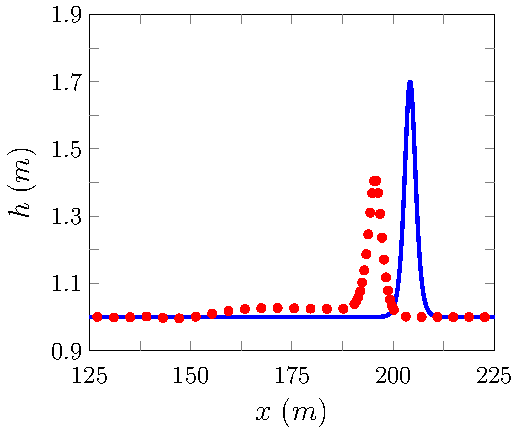
\includegraphics[width=\textwidth]{../chp5/figures/Analytic/Soliton/Example/FDVM1.pdf}
		\subcaption{$\text{FDVM}_1$}
		\vspace{0.5cm}
	\end{subfigure}%
	\begin{subfigure}{0.5\textwidth}
		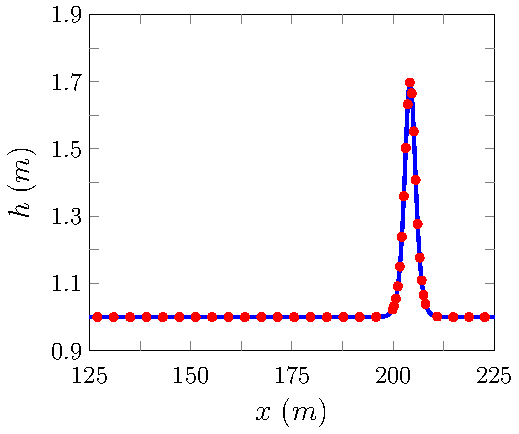
\includegraphics[width=\textwidth]{../chp5/figures/Analytic/Soliton/Example/FDVM2.pdf}
		\subcaption{$\text{FDVM}_2$}
		\vspace{0.5cm}
	\end{subfigure}
	\begin{subfigure}{0.5\textwidth}
		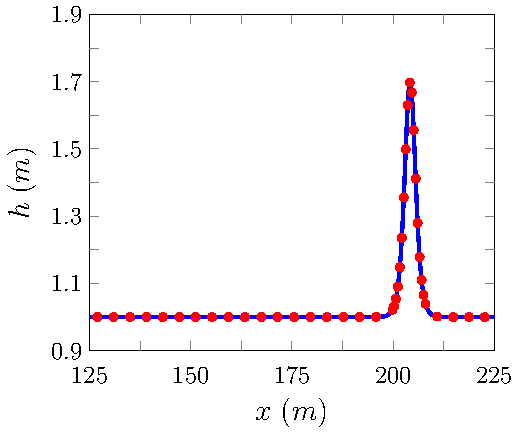
\includegraphics[width=\textwidth]{../chp5/figures/Analytic/Soliton/Example/FEVM2.pdf}
		\subcaption{$\text{FEVM}_2$}
		\vspace{0.5cm}
	\end{subfigure}%
	\begin{subfigure}{0.5\textwidth}
		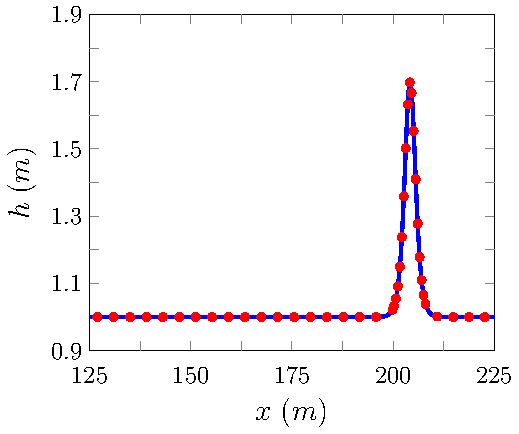
\includegraphics[width=\textwidth]{../chp5/figures/Analytic/Soliton/Example/FDVM3.pdf}
		\subcaption{$\text{FDVM}_3$}
		\vspace{0.5cm}
	\end{subfigure}
	\begin{subfigure}{0.5\textwidth}
		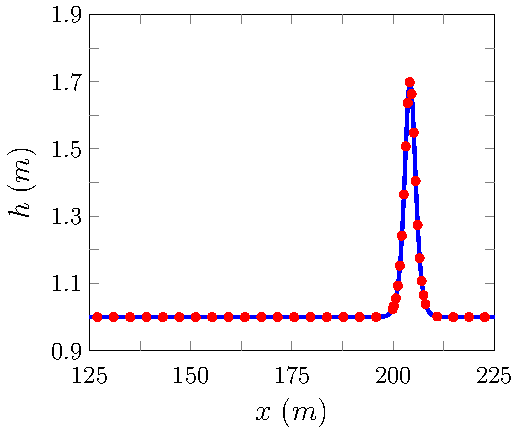
\includegraphics[width=\textwidth]{../chp5/figures/Analytic/Soliton/Example/D.pdf}
		\subcaption{$\mathcal{D}$}
		\vspace{0.5cm}
	\end{subfigure}%
	\begin{subfigure}{0.5\textwidth}
		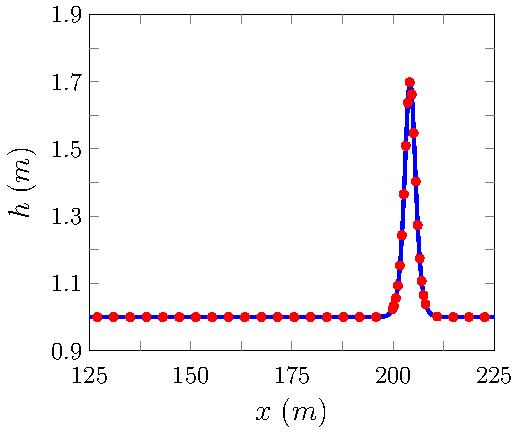
\includegraphics[width=\textwidth]{../chp5/figures/Analytic/Soliton/Example/W.pdf}
		\subcaption{$\mathcal{W}$}
		\vspace{0.5cm}
	\end{subfigure}
	\caption{Comparison of the analytic solution ({\color{blue} \solidrule}) and numerical solution with $\Delta x = {100} / {2^{11}}m$ ({\color{red} $\bullet$}) for the soliton problem at $t=50s$ for all methods.}
	\label{fig:SolitonExAll}
\end{figure}
	
\begin{figure}
	\centering
	\begin{subfigure}{0.5\textwidth}
		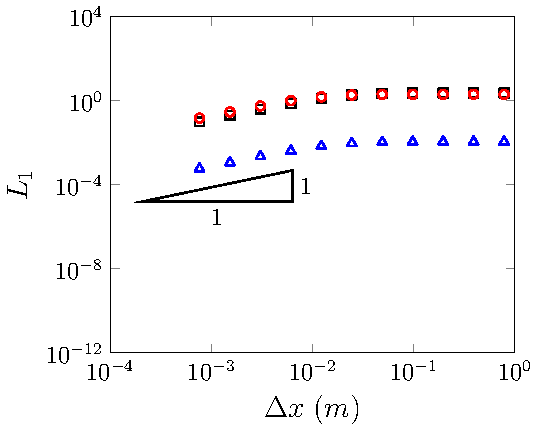
\includegraphics[width=\textwidth]{../chp5/figures/Analytic/Soliton/L1/FDVM1N.pdf}
		\subcaption{$\text{FDVM}_1$}
		\vspace{0.5cm}
	\end{subfigure}%
	\begin{subfigure}{0.5\textwidth}
		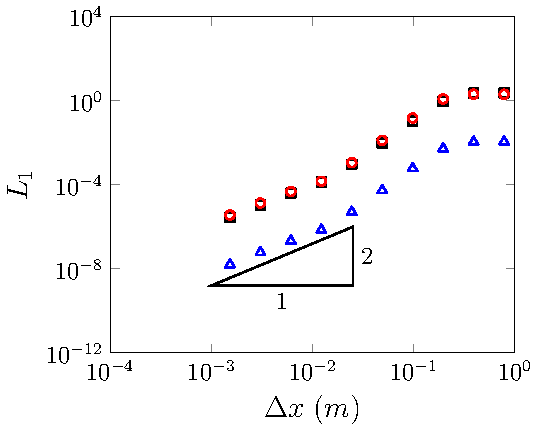
\includegraphics[width=\textwidth]{../chp5/figures/Analytic/Soliton/L1/FDVM2N.pdf}
		\subcaption{$\text{FDVM}_2$}
		\vspace{0.5cm}
	\end{subfigure}
	\begin{subfigure}{0.5\textwidth}
		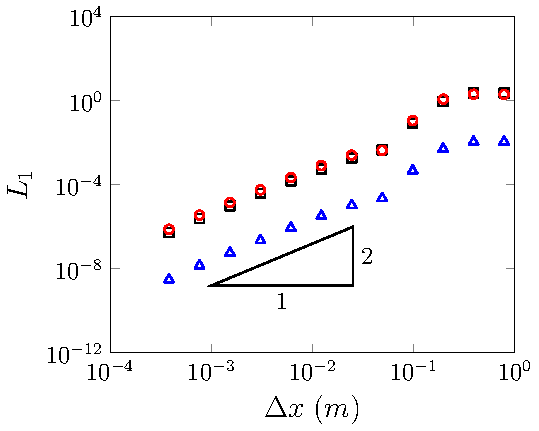
\includegraphics[width=\textwidth]{../chp5/figures/Analytic/Soliton/L1/FEVM2.pdf}
		\subcaption{$\text{FEVM}_2$}
		\vspace{0.5cm}
	\end{subfigure}%
	\begin{subfigure}{0.5\textwidth}
		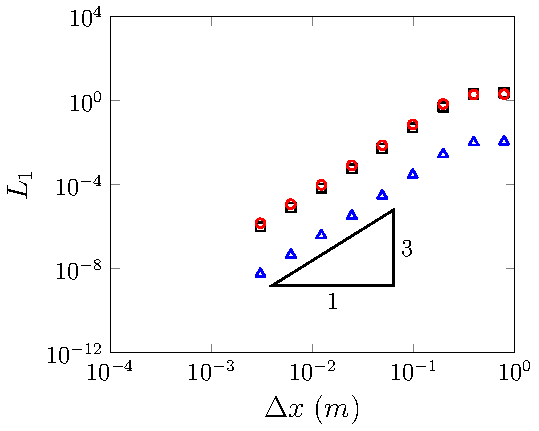
\includegraphics[width=\textwidth]{../chp5/figures/Analytic/Soliton/L1/FDVM3N.pdf}
		\subcaption{$\text{FDVM}_3$}
		\vspace{0.5cm}
	\end{subfigure}
	\begin{subfigure}{0.5\textwidth}
		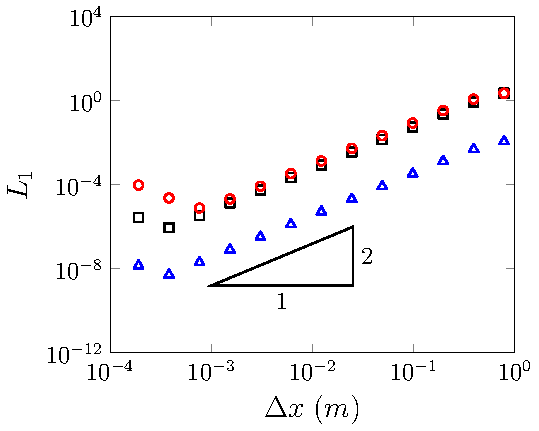
\includegraphics[width=\textwidth]{../chp5/figures/Analytic/Soliton/L1/D.pdf}
		\subcaption{$\mathcal{D}$}
		\vspace{0.5cm}
	\end{subfigure}%
	\begin{subfigure}{0.5\textwidth}
		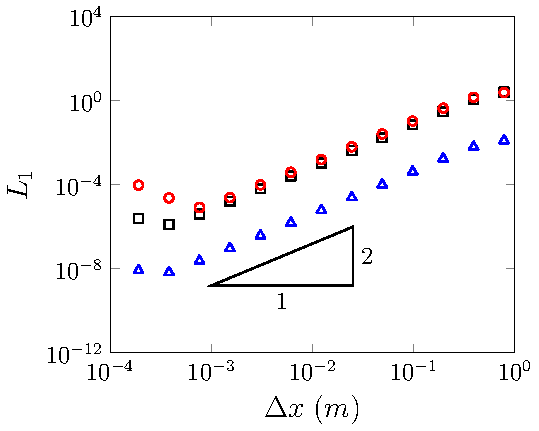
\includegraphics[width=\textwidth]{../chp5/figures/Analytic/Soliton/L1/W.pdf}
		\subcaption{$\mathcal{W}$}
		\vspace{0.5cm}
	\end{subfigure}
	\caption{Convergence plots as measured by the $L_1$ norm for $h$ (\trianglet{blue}), $u$ (\squaret{black}) and $G$ (\circlet{red}) for the soliton problem for all methods.}
	\label{fig:SolitonL1All}
\end{figure}
	
\begin{figure}
	\centering
	\begin{subfigure}{0.5\textwidth}
		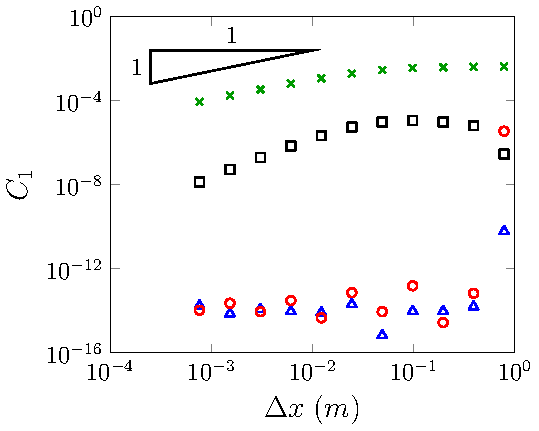
\includegraphics[width=\textwidth]{../chp5/figures/Analytic/Soliton/C1/FDVM1N.pdf}
		\subcaption{$\text{FDVM}_1$}
		\vspace{0.5cm}
	\end{subfigure}%
	\begin{subfigure}{0.5\textwidth}
		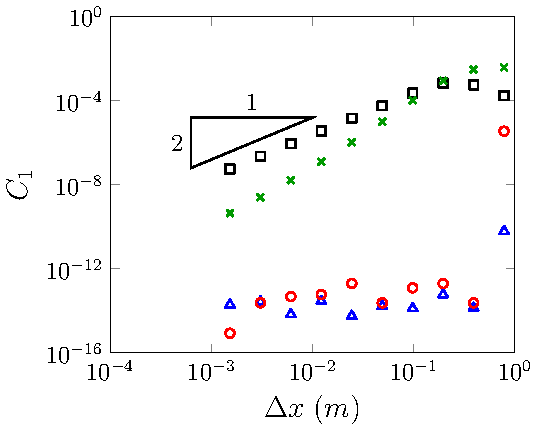
\includegraphics[width=\textwidth]{../chp5/figures/Analytic/Soliton/C1/FDVM2N.pdf}
		\subcaption{$\text{FDVM}_2$}
		\vspace{0.5cm}
	\end{subfigure}
	\begin{subfigure}{0.5\textwidth}
		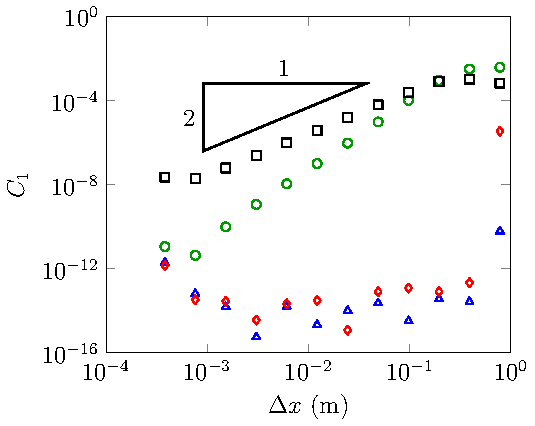
\includegraphics[width=\textwidth]{../chp5/figures/Analytic/Soliton/C1/FEVM2.pdf}
		\subcaption{$\text{FEVM}_2$}
		\vspace{0.5cm}
	\end{subfigure}%
	\begin{subfigure}{0.5\textwidth}
		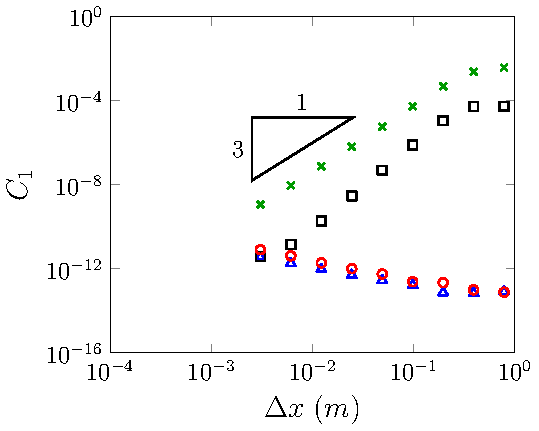
\includegraphics[width=\textwidth]{../chp5/figures/Analytic/Soliton/C1/FDVM3N.pdf}
		\subcaption{$\text{FDVM}_3$}
		\vspace{0.5cm}
	\end{subfigure}
	\begin{subfigure}{0.5\textwidth}
		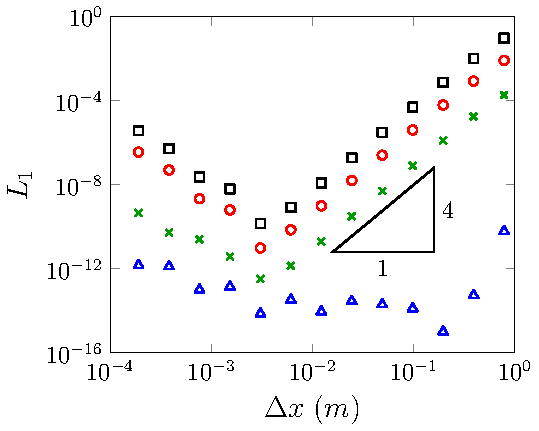
\includegraphics[width=\textwidth]{../chp5/figures/Analytic/Soliton/C1/D.pdf}
		\subcaption{$\mathcal{D}$}
		\vspace{0.5cm}
	\end{subfigure}%
	\begin{subfigure}{0.5\textwidth}
		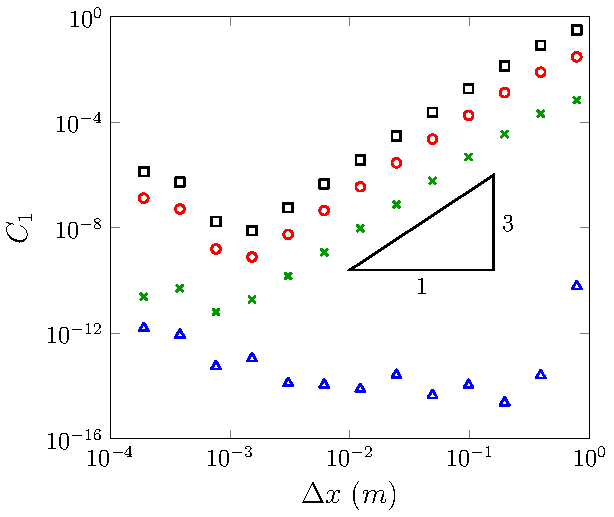
\includegraphics[width=\textwidth]{../chp5/figures/Analytic/Soliton/C1/W.pdf}
		\subcaption{$\mathcal{W}$}
		\vspace{0.5cm}
	\end{subfigure}
	\caption{Conservation plots as measured by $C_1$ for $h$ (\trianglet{blue}), $uh$ (\squaret{black}), $G$ (\diamondt{red}) and $\mathcal{H}$ ({\color{green!60!black}$\times$}) for the soliton problem for all methods.}
	\label{fig:SolitonC1All}
\end{figure}


\begin{figure}
	\centering
	\begin{subfigure}{0.5\textwidth}
		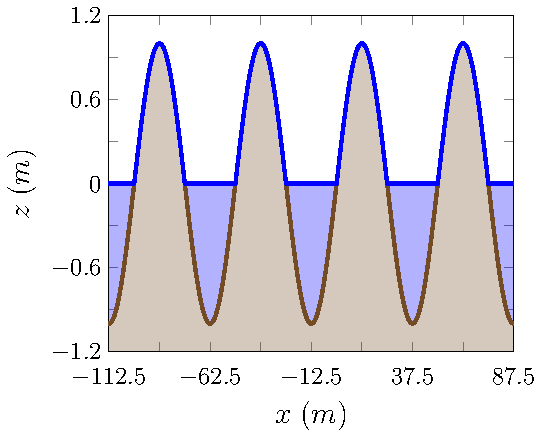
\includegraphics[width=\textwidth]{../chp5/figures/Analytic/LakeAtRest/Example/FEVMWB.pdf}
		\subcaption{$\text{FEVM}_2$ well balanced}
		\vspace{0.5cm}
	\end{subfigure}%
	\begin{subfigure}{0.5\textwidth}
		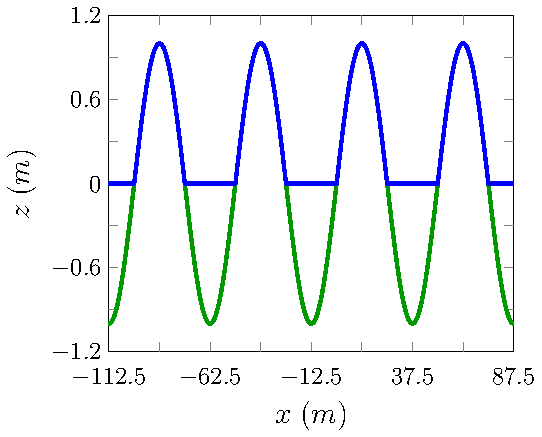
\includegraphics[width=\textwidth]{../chp5/figures/Analytic/LakeAtRest/Example/FEVMnWB.pdf}
		\subcaption{$\text{FEVM}_2$ not well balanced}
		\vspace{0.5cm}
	\end{subfigure}
	\begin{subfigure}{0.5\textwidth}
		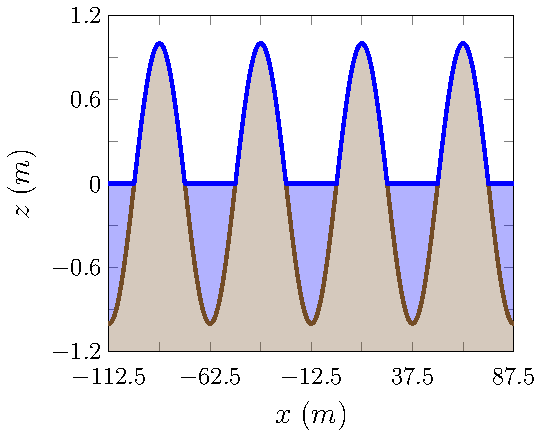
\includegraphics[width=\textwidth]{../chp5/figures/Analytic/LakeAtRest/Example/FDVMWB.pdf}
		\subcaption{$\text{FDVM}_2$ well balanced}
		\vspace{0.5cm}
	\end{subfigure}%
	\begin{subfigure}{0.5\textwidth}
		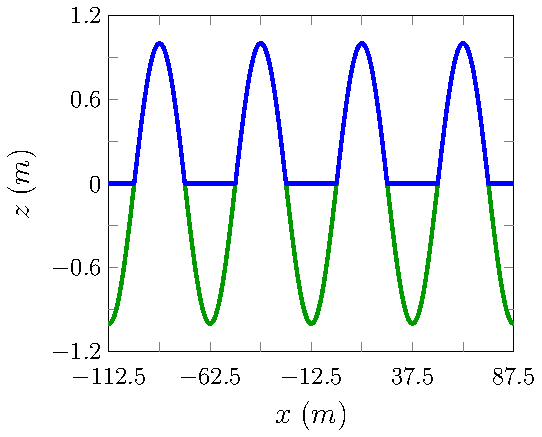
\includegraphics[width=\textwidth]{../chp5/figures/Analytic/LakeAtRest/Example/FDVMnWB.pdf}
		\subcaption{$\text{FDVM}_2$ not well balanced}
		\vspace{0.5cm}
	\end{subfigure}
	\caption{Comparison of the analytic solution ({\color{red} \solidrule}) and numerical solution with $\Delta x = {100} / {2^{10}}m$ ({\color{blue} \solidrule}) for the lake at rest problem at $t=10s$ for all methods.}
	\label{fig:LakeAtRestEx}
\end{figure}

\begin{figure}
	\centering
	\begin{subfigure}{0.5\textwidth}
		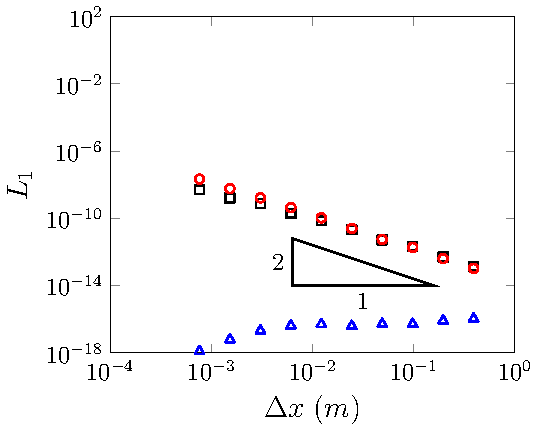
\includegraphics[width=\textwidth]{../chp5/figures/Analytic/LakeAtRest/L1/FEVMWB.pdf}
		\subcaption{$\text{FEVM}_2$ well balanced}
		\vspace{0.5cm}
	\end{subfigure}%
	\begin{subfigure}{0.5\textwidth}
		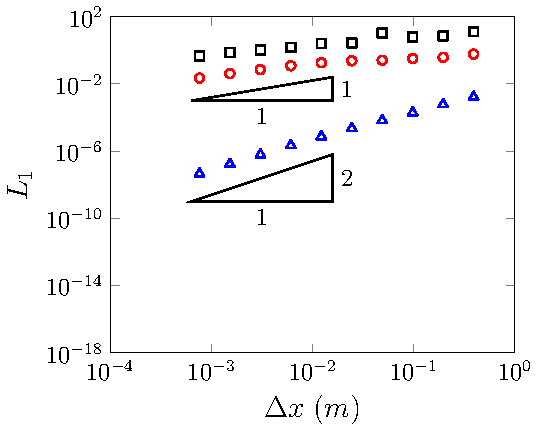
\includegraphics[width=\textwidth]{../chp5/figures/Analytic/LakeAtRest/L1/FEVMnWB.pdf}
		\subcaption{$\text{FEVM}_2$ not well balanced}
		\vspace{0.5cm}
	\end{subfigure}
	\begin{subfigure}{0.5\textwidth}
		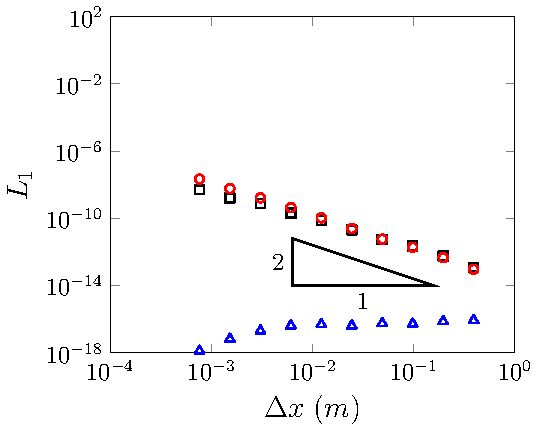
\includegraphics[width=\textwidth]{../chp5/figures/Analytic/LakeAtRest/L1/FDVMWB.pdf}
		\subcaption{$\text{FDVM}_2$ well balanced}
		\vspace{0.5cm}
	\end{subfigure}%
	\begin{subfigure}{0.5\textwidth}
		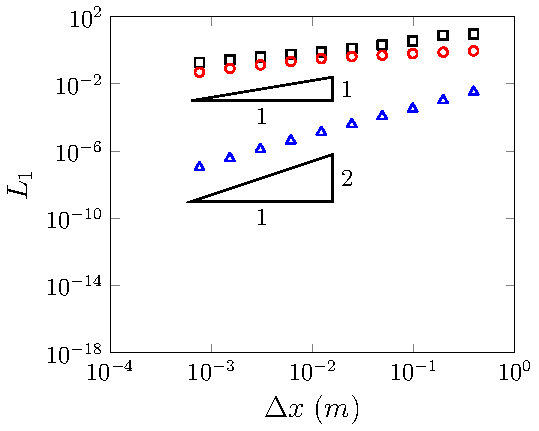
\includegraphics[width=\textwidth]{../chp5/figures/Analytic/LakeAtRest/L1/FDVMnWB.pdf}
		\subcaption{$\text{FDVM}_2$ not well balanced}
		\vspace{0.5cm}
	\end{subfigure}
	\caption{Convergence plots as measured by the $L_1$ norm for $h$ (\trianglet{blue}), $u$ (\squaret{black}) and $G$ (\diamondt{red}) for the lake at rest problem at $t=10s$ for all methods.}
	\label{fig:LakeAtRestEL1}
\end{figure}

\begin{figure}
	\centering
	\begin{subfigure}{0.5\textwidth}
		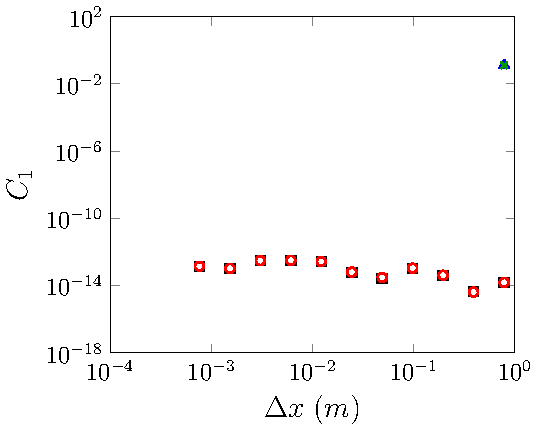
\includegraphics[width=\textwidth]{../chp5/figures/Analytic/LakeAtRest/C1/FEVMWB.pdf}
		\subcaption{$\text{FEVM}_2$ well balanced}
		\vspace{0.5cm}
	\end{subfigure}%
	\begin{subfigure}{0.5\textwidth}
		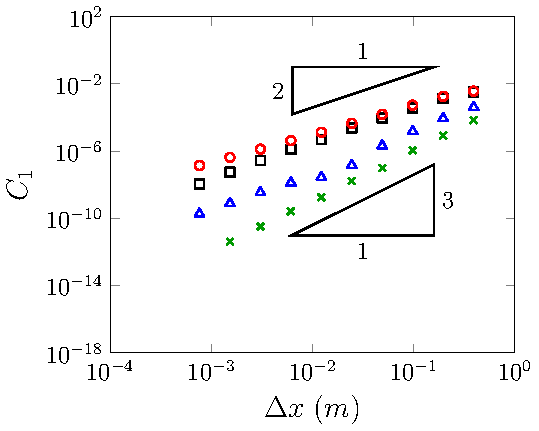
\includegraphics[width=\textwidth]{../chp5/figures/Analytic/LakeAtRest/C1/FEVMnWB.pdf}
		\subcaption{$\text{FEVM}_2$ not well balanced}
		\vspace{0.5cm}
	\end{subfigure}
	\begin{subfigure}{0.5\textwidth}
		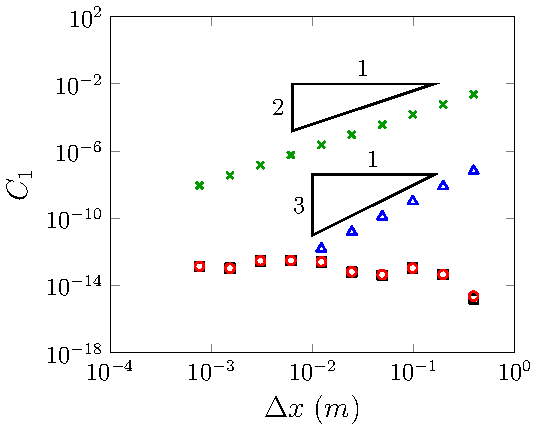
\includegraphics[width=\textwidth]{../chp5/figures/Analytic/LakeAtRest/C1/FDVMWB.pdf}
		\subcaption{$\text{FDVM}_2$ well balanced}
		\vspace{0.5cm}
	\end{subfigure}%
	\begin{subfigure}{0.5\textwidth}
		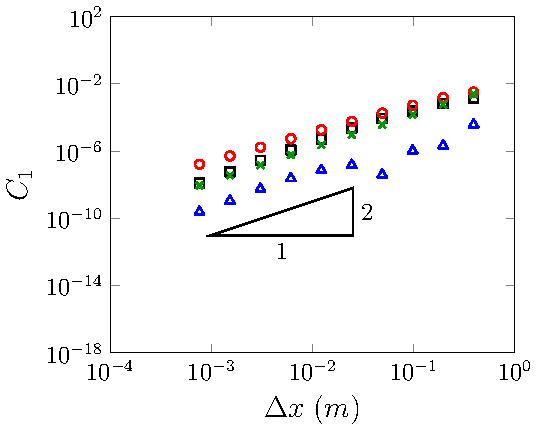
\includegraphics[width=\textwidth]{../chp5/figures/Analytic/LakeAtRest/C1/FDVMnWB.pdf}
		\subcaption{$\text{FDVM}_2$ not well balanced}
		\vspace{0.5cm}
	\end{subfigure}
	\caption{Error in conservation plots as measured by the $C_1$ norm for $h$ (\trianglet{blue}), $u$ (\squaret{black}) and $G$ (\diamondt{red}) for the lake at rest problem at $t=10s$ for all methods.}
	\label{fig:LakeAtRestEC1}
\end{figure}
\end{document}